% ============================================================
%  Vibe Slicer – Scientific Paper
%  ASE S2026, University of Salzburg
%  Thomas Martin Pfister
% ============================================================
\documentclass[10pt,twocolumn,a4paper]{article}

% ---- Fonts & encoding ----
\usepackage[T1]{fontenc}
\usepackage[utf8]{inputenc}
\usepackage{mathptmx}          % Times New Roman body + math

% ---- Page geometry (ACM POPL / IEEE-style margins) ----
\usepackage[a4paper,
            top=2.5cm, bottom=2.5cm,
            left=1.8cm, right=1.8cm,
            columnsep=0.6cm]{geometry}

% ---- Typography ----
\usepackage{microtype}
\usepackage{setspace}

% ---- Section headings: bold, slightly larger, no numbering gap ----
\usepackage{titlesec}
\titleformat{\section}{\normalfont\large\bfseries}{\thesection.}{0.5em}{}
\titleformat{\subsection}{\normalfont\normalsize\bfseries\itshape}{\thesubsection}{0.5em}{}
\titlespacing*{\section}{0pt}{8pt plus 2pt minus 1pt}{4pt plus 1pt}
\titlespacing*{\subsection}{0pt}{6pt plus 1pt minus 1pt}{2pt plus 1pt}

% ---- Floats & tables ----
\usepackage{booktabs}
\usepackage{multirow}
\usepackage{array}
\usepackage{longtable}
\usepackage{caption}
\captionsetup{font=small, labelfont=bf, skip=4pt}
\usepackage{float}
\usepackage{graphicx}

% ---- Math ----
\usepackage{amsmath}

% ---- URLs / hyperlinks ----
\usepackage{url}
\usepackage[hidelinks]{hyperref}

% ---- Code listings ----
\usepackage{listings}
\lstset{basicstyle=\ttfamily\footnotesize, breaklines=true,
        frame=single, framesep=2pt, xleftmargin=4pt}

% ---- Misc ----
\usepackage{textcomp}
\usepackage{xspace}
\usepackage{enumitem}
\setlist{noitemsep, topsep=2pt}

% ---- Compact abstract ----
\renewenvironment{abstract}{%
  \small\textbf{Abstract---}\ignorespaces}{\par}

% ---- No date ----
\date{}

% ============================================================
\begin{document}

% ---- Title block ----
\twocolumn[{%
\begin{center}
  {\LARGE\bfseries Can AI Develop a Slicer?\\[4pt]
   Developing and Evaluating an FDM 3D Printer Slicer\\[2pt]
   Built Using Only AI Tools Without Slicer-Development Experience}\\[10pt]
  {\large Thomas Martin Pfister}\\[2pt]
  {\normalsize Department of Computer Science, University of Salzburg, Austria}\\
  {\normalsize \texttt{thomas.pfister@stud.plus.ac.at}}\\[8pt]
\end{center}

\begin{abstract}
Slicing software translates three-dimensional mesh models into
layer-by-layer G-code instructions for Fused Deposition Modeling (FDM) printers.
Developing such software has traditionally demanded deep expertise in
computational geometry, toolpath planning, and manufacturing processes.
This paper investigates whether contemporary AI-assisted development
can produce a functionally correct slicer when the developer is an
experienced FDM user—familiar with 3D printers, G-code, and consumer grade slicers such as
Cura—but has \emph{no} experience in slicer development or
geometric computing.
The resulting prototype—\emph{Vibe Slicer}—implements a complete
STL-to-G-code pipeline in Go, including contour hierarchy extraction
with hole support, configurable wall lines, solid top/bottom layers,
zig-zag infill, skirt, brim, retraction, and cooling fan control.
Vibe Slicer is benchmarked against Ultimaker Cura on two reference
objects—a 10\,mm cube and a 40$\times$40$\times$5\,mm plate with
two circular holes—measuring slicing time, print time,
and dimensional accuracy both theoretically and through physical prints.
The benchmarks showed that theoretical accuracy is identical to Cura;
practical accuracy under matched parameters is within $\pm$0.3\,mm for outer dimensions and within $\pm$0.2\,mm for holes.
Print time diverges by up to 62\,\% due to differences in toolpath
optimisation, and slicing time is too small to measure meaningfully for both tools on the
tested geometry.
The work demonstrates that AI-assisted development can lower
the barrier of entry for computationally complex domains, while
also exposing robustness limits inherent in LLM-generated geometry algorithms.
\end{abstract}

\vspace{6pt}
\noindent\textbf{Keywords---} 3D printing; FDM slicer;
AI-assisted development; large language models; G-code;
computational geometry; STL; Ultimaker Cura
\vspace{10pt}
}]

% ============================================================
\section{Introduction}
% ============================================================

Fused Deposition Modeling (FDM) is the most widely deployed form
of desktop additive manufacturing~\cite{guo2013additive}.
Central to every FDM workflow is a \emph{slicer}: software that
decomposes a three-dimensional mesh into planar cross-sections,
generates perimeter toolpaths, computes fill patterns,
and serialises the result as G-code—a standardised numerical
control language understood by printer firmware.
Mature, open-source slicers such as Ultimaker Cura~\cite{cura}
and PrusaSlicer~\cite{prusaslicer} are the product of years
of engineering effort, encoding substantial expertise in polygon
offsetting, contour stitching, and extrusion calibration.

The rapid advancement of large language model (LLM) code-generation
capabilities has prompted widespread discussion about whether AI
assistance can replace or complement specialist knowledge in software
engineering~\cite{chen2021codex,jiang2023survey}.
Yet little empirical work examines whether LLM assistance suffices
for niche domains that require non-trivial algorithmic knowledge.

This paper addresses that gap through a concrete experiment:
the development of a complete FDM slicer—\emph{Vibe Slicer}—
using exclusively AI-assisted code generation.
The author is an experienced FDM user—familiar with operating
3D printers, reading and modifying G-code, and using the Cura
slicer—but has no prior experience in developing a slicer or in
geometric computing more broadly. This profile is deliberate:
it isolates the question of whether AI assistance can bridge the
\emph{implementation} gap (the algorithms and geometry) for a
practitioner who already understands the \emph{problem domain}
(what a slicer must produce and why).
Two research questions drive the work:

\begin{enumerate}[label=\textbf{RQ\arabic*.}]
  \item \textbf{Feasibility.} Can an experienced FDM user with no
        slicer-development or geometric-computing experience produce
        a functionally correct STL-to-G-code slicer relying
        exclusively on AI-assisted code generation?
  \item \textbf{Comparative Performance.} How do the dimensional
        accuracy and efficiency of an AI-developed slicer compare to a
        mature reference implementation (Cura) on identical inputs?
\end{enumerate}

The remainder of the paper is structured as follows.
Section~\ref{sec:related} reviews related work.
Section~\ref{sec:slicer} describes what a slicer is and does.
Section~\ref{sec:stl} explains the STL file format.
Section~\ref{sec:design} presents the design and implementation of Vibe Slicer.
Section~\ref{sec:eval} defines the experimental methodology and reports results.
Section~\ref{sec:discussion} discusses findings and limitations.
Section~\ref{sec:conclusion} concludes.

% ============================================================
\section{Related Work}
\label{sec:related}
% ============================================================

\subsection{FDM Slicing Software}

Converting a triangulated surface mesh into planar cross-sections
is computationally straightforward at the triangle-plane intersection
level, but robust contour stitching—merging unordered intersection
segments into closed loops while handling degenerate geometry—requires
careful attention to floating-point tolerances~\cite{gibson2021additive}.
Polygon offsetting, used to generate inset wall lines, is generally
approached through the Clipper library~\cite{clipper2}, which applies
integer arithmetic and Minkowski sum approximations.
Production slicers such as Cura implement sophisticated algorithms
for seam placement, variable-width extrusion, support structure
generation, and multi-material routing that go far beyond the scope
of this work.

\subsection{AI-Assisted Software Development}

LLMs have been applied to code generation since at least GPT-2~\cite{radford2019gpt2},
but gained broad practitioner adoption with GitHub Copilot~\cite{copilot}
and GPT-4~\cite{openai2023gpt4}.
Chen~et~al.~\cite{chen2021codex} introduced the HumanEval benchmark
and showed that GPT-4-class models achieve over 80\,\% pass@1
on standard algorithmic problems.
Jimenez~et~al.~\cite{jimenez2023swebench} introduced SWE-bench
for repository-scale repair, where models perform substantially worse.
Survey studies~\cite{ziegler2022productivity} report that developers
perceive AI assistance as most valuable for boilerplate and
moderately helpful for algorithmic tasks, but insufficient for
novel or domain-specific problems without human oversight.
The present work contributes an empirical data point: a sustained,
end-to-end development effort in a domain requiring non-trivial
algorithmic knowledge.

\subsection{Evaluation of AI-Generated Systems}

To the best of the author's knowledge, no prior work directly
evaluates an LLM-generated slicer against a production reference.
Closest in spirit are studies surveying LLM code-generation capability~\cite{jiang2023survey}.
This paper extends that line of work to a full software artifact
with real hardware evaluation.

\subsection{Prompt Engineering and Iterative Refinement}

A key practical finding in the LLM-assisted development literature
is that the quality of generated code depends strongly on the
specificity and structure of the prompt~\cite{ziegler2022productivity}.
Simple one-line prompts tend to produce working but brittle
implementations, while multi-constraint prompts
(listing requirements, edge cases, and expected output format
explicitly) produce more robust code at the cost of longer
context windows and higher token usage.
This trade-off was directly observed during Vibe Slicer's
development: early one-line or short prompts (e.g., S1 - \emph{``Create a go file that takes a file in STL format as input, slices the object in the STL file every 0.2mm, starting from the bottom and converts the resulting 2D coordinates into an array of x and y
coordinates.''}) produced a running prototype within minutes
but with a subtle bug (8 outside edge points per layer on a cube instead of 4)
that required three additional prompts (S2, S3 and S4) to diagnose and resolve.
Later, more detailed multi-constraint prompts (S6 - spanning 16 lines
of explicit requirements for the contour pipeline refactor)
produced more reliable results in fewer iterations, at the cost
of substantially more prompt-writing effort from the developer.

% ============================================================
\section{What Is a Slicer?}
\label{sec:slicer}
% ============================================================

A slicer is a software tool that converts a 3D model into machine
instructions for an FDM printer~\cite{gibson2021additive}.
The high-level task appears straightforward: cut the model into
horizontal layers and tell the printer where to move and how much
material to extrude on each layer.
In practice, however, a slicer must solve several interlocking
subproblems.

\textbf{Layer slicing.}
The model geometry is intersected at uniform $z$-intervals
(the \emph{layer height}) to produce a set of 2D cross-sections
per layer. Each cross-section is a collection of line segments
derived from triangle-plane intersections.

\textbf{Contour extraction.}
Unordered intersection segments must be stitched into ordered,
closed contour loops. Correct winding (clockwise for outer
boundaries, counter-clockwise for holes) is essential for
subsequent offset and fill operations.

\textbf{Wall generation.}
The outermost contour is printed as the outer wall.
Additional inner wall lines are generated by \emph{inward offsetting}
(shrinking) the contour by one line width per pass.

\textbf{Fill generation.}
The area bounded by the innermost wall is filled with a dense
pattern for solid layers (floor and ceiling) or a sparse pattern
for infill. Alternating $\pm45^{\circ}$ diagonal hatching is standard.

\textbf{G-code serialisation.}
Toolpaths are converted to G-code: linear move commands
(\texttt{G0} and \texttt{G1}) with $X$, $Y$, $Z$ coordinates, feedrate value ($F$) and extrusion position ($E$),
temperature commands (\texttt{M104}, \texttt{M109}, \texttt{M140}, \texttt{M190} and \texttt{M105}),
fan control (\texttt{M106} and \texttt{M107}), and retraction moves.
Extrusion volumes are derived from line cross-section area
and segment length divided by filament cross-sectional area.

Together these sub-problems span computational geometry,
numerical analysis, and domain-specific manufacturing knowledge—making
a slicer a suitable and challenging test case for AI-assisted
development.

\begin{figure}[t]
\centering
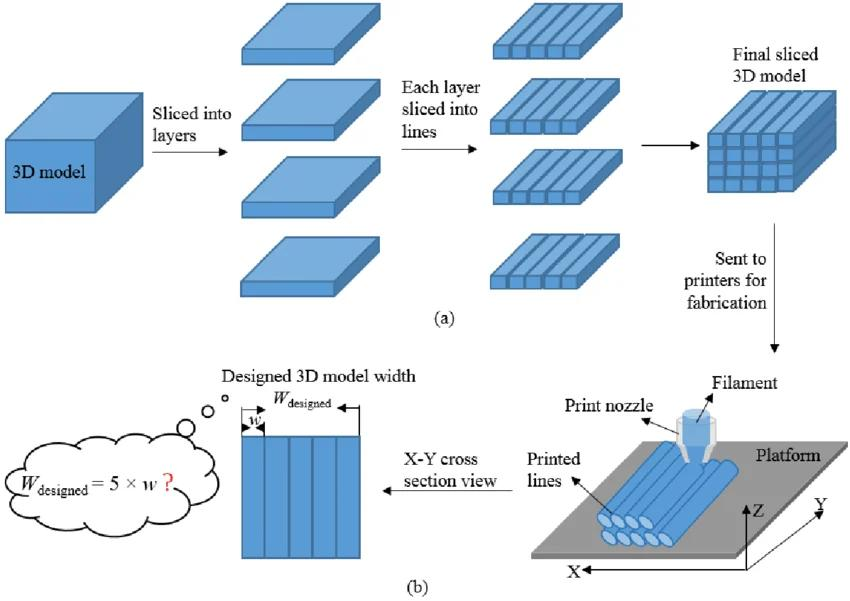
\includegraphics[width=\columnwidth]{slicer_process.pdf}
\caption{The FDM slicing and fabrication process.
(a) A 3D model is sliced into layers, each layer is sliced into
lines, and the result is sent to the printer.
(b) During fabrication the nozzle deposits printed lines whose
combined width must reconstruct the designed model width.
Figure reproduced from Jin~et~al.~\cite{jin2020connections}
(CC~BY~4.0).}
\label{fig:slicing}
\end{figure}

Figure~\ref{fig:slicing} illustrates the full pipeline from
mesh to printed lines.

% ============================================================
\section{The STL File Format}
\label{sec:stl}
% ============================================================

Stereolithography (STL) is the de-facto standard exchange format
for 3D printer meshes~\cite{gibson2021additive}.
An STL file represents a closed triangular mesh as a flat list
of triangles, each defined by its three vertex coordinates
and a surface normal vector. There is no topological adjacency
information: the mesh is purely a soup of independent triangles.

STL files exist in two variants. \emph{Binary} STL encodes
triangles as packed 32-bit floats preceded by a 4-byte triangle
count header, enabling $O(1)$ size validation before parsing.
\emph{ASCII} STL uses a line-by-line text representation readable
by humans but substantially larger on disk.
Listing~\ref{lst:ascii_stl} shows the ASCII representation
of a single triangle.

\begin{lstlisting}[caption={ASCII STL representation of one triangle.},
                   label={lst:ascii_stl}, language={}]
facet normal 0 0 -1
  outer loop
    vertex 0 0 0
    vertex 10 0 0
    vertex 10 10 0
  endloop
endfacet
\end{lstlisting}

The absence of topological information is the core challenge
for slicer development: contour stitching must reconstruct
connectivity solely from the coincidence of triangle edge endpoints,
making floating-point tolerances critical to correctness.
For instance, two triangles sharing an edge in theory share
exactly two vertex coordinate pairs; in practice, STL files
produced by different CAD tools may represent nominally identical
coordinates with slightly different float representations,
requiring tolerance-based snapping before graph construction.

\subsection*{Triangle–Plane Intersection}

For a given layer at height $z_k$, a triangle contributes an
intersection segment if and only if the three vertices are not all
on the same side of the plane $z = z_k$.
Letting vertex heights be $z_a, z_b, z_c$, the cases are:

\begin{enumerate}
  \item All three vertices satisfy $z_i \approx z_k$ (\emph{coplanar}):
        all three edges are emitted as segments.
  \item Exactly one vertex lies above and two below (or vice versa):
        the two crossing edges are linearly interpolated to find the
        two intersection points forming the segment.
  \item All vertices on the same side: no intersection.
\end{enumerate}

The interpolation parameter $t$ along an edge from $\mathbf{v}_0$
to $\mathbf{v}_1$ is:
\begin{equation}
  t = \frac{z_k - z_{v_0}}{z_{v_1} - z_{v_0}}, \quad
  \mathbf{p} = \mathbf{v}_0 + t\,(\mathbf{v}_1 - \mathbf{v}_0).
\end{equation}

Vibe Slicer implements all three cases, with the coplanar case
handled by emitting all three edges and relying on shared-edge
cancellation during graph construction—a fix identified during
prompt~S8 of the development log that resolved a top-surface
artefact on the cube test object.

% ============================================================
\section{Vibe Slicer: Design \& Implementation}
\label{sec:design}
% ============================================================

\subsection{Development Methodology}

The author's relevant background is that of an experienced FDM
practitioner: familiar with operating consumer FDM printers,
reading and hand-editing G-code, and configuring prints in the
Cura slicer. Critically, however, the author had never developed
a slicer, implemented a computational-geometry algorithm, or
worked with mesh-processing code before this project. This means
the author could readily judge whether the \emph{output} of the
slicer was correct (e.g., recognising a malformed toolpath or an
incorrect extrusion command in the G-code) while having no prior
basis for implementing the \emph{algorithms} that produce it.

Vibe Slicer was developed over the course of the Summer 2026
semester using two AI assistants: GPT-5.3 Codex for the early
development phase, and GPT-5.4-mini for the later phase. The
transition between the two models was not a deliberate
methodological choice but was forced by GPT-5.3 Codex being
removed from GitHub Copilot partway through the project; all
subsequent prompts were therefore issued to GPT-5.4-mini.
The author provided high-level requirements and iterative
feedback in natural language; all algorithmic code was generated
and refined through conversational prompting.
No slicer textbooks, computational-geometry references, geometry
libraries, or existing slicer source code were consulted during
development; the author's FDM domain knowledge was used only to
specify requirements and to evaluate output correctness.
The implementation language is Go (v1.22), chosen for its
performance characteristics and straightforward single-binary
deployment. The project comprises approximately 2\,700 lines of
code across two main source files and their associated test suites.

The 44 prompts documented in Table~\ref{tab:prompts_full}
(8 for the STL-to-JSON converter and 36 for the G-code generator)
are only those that contributed directly to the final result;
they are a curated subset of the development effort rather than a
complete transcript. In total, well over 150 prompts were issued.
The majority are not recorded because they led to unproductive
cycles in which a fix for one problem introduced a regression
elsewhere—correcting a contour artefact would break the infill,
repairing the infill would distort a wall, and so on—after which
the working tree was reset to a known-good state and the approach
re-attempted. Only the prompts on the path that produced the
final, working code are retained here. Of the 36 recorded G-code
prompts, 22 (G1--G22) correspond to features present in the final
code, while the remainder (G23--G36) belong to a hierarchy-aware
offset refactor that was never completed (see below). Several
recorded prompts still required multiple rounds of back-and-forth
when the generated code introduced new bugs, most notably during
contour stitching (prompts S5--S8 in the converter) and polygon
offsetting (prompts G23--G36 in the generator, which were ultimately
abandoned due to token budget exhaustion).

\subsection{Two-Step Pipeline}

The pipeline is divided into two independent command-line tools
to maintain a clean separation of concerns.
The first tool, \texttt{stl\_to\_json\_converter}, reads an
STL file and produces a structured JSON representation of the
sliced layers, including a full contour hierarchy.
The second tool, \texttt{create\_g\_code}, consumes the JSON
and emits a printer-ready G-code file.
This architecture facilitates independent testing of each stage.

\subsection{JSON Intermediate Representation}

The intermediate JSON format is the key interface between the
two pipeline stages. Each layer entry records the $z$ height,
a legacy flat \texttt{points} array retained for backward
compatibility, and a \texttt{contours} array that encodes the
full contour hierarchy with children (holes) nested recursively.
Listing~\ref{lst:json} shows the schema for a single layer
of the cube\_10 object.
\newpage
\begin{lstlisting}[caption={JSON intermediate format: one layer
                   of cube\_10 (4-point outer contour, no holes).},
                   label={lst:json}, language={}]
{
  "z": 0.2,
  "points": [
    {"x": 0.0, "y": 0.0},
    {"x": 0.0, "y": 10.0},
    {"x": 10.0, "y": 10.0},
    {"x": 10.0, "y": 0.0}
  ],
  "contours": [{
    "kind": "outer",
    "points": [
      {"x":0.0,"y":0.0},{"x":0.0,"y":10.0},
      {"x":10.0,"y":10.0},{"x":10.0,"y":0.0}
    ],
    "children": []
  }]
}
\end{lstlisting}

For the Hole\_Structure, each layer's \texttt{contours} array
contains one outer contour with two hole children, one per
circular through-hole.
The G-code generator traverses this hierarchy: outer contours
drive wall printing, and hole children reverse the winding
so the printer correctly traverses the inner boundary of each
circular hole.

\subsection{Usage}

The two-step workflow can be invoked from the command line in two different ways as follows:

\begin{lstlisting}[caption={Two-step CLI workflow with included parameters.},
                   label={lst:workflow}, language={}]
go run ./stl_to_json_converter \
  -in cube_10.stl -layer 0.2 -out slices.json

go run ./create_g_code \
  -json-in slices.json -gcode-out print.gcode \
  -offset-x 195 -offset-y 195 \
  -outer-wall-lines 3 -solid-bottom-layers 3 \
  -solid-top-layers 3 -infill true \
  -infill-density 25 -cooling-fan true \
  -print-temp 205 -bed-temp 60 \
  -print-speed 30
\end{lstlisting}
The parameters can also be hard coded into the source code and then do not need to be specified in the invocation:

\begin{lstlisting}[caption={Two-step CLI workflow without included parameters.},
	label={lst:workflow2}, language={}]
go run ./stl_to_json_converter \
  -in cube_10.stl -layer 0.2 -out slices.json
	
go run ./create_g_code \
  -json-in slices.json -gcode-out print.gcode
\end{lstlisting}

\subsection{STL Parsing}

Both binary and ASCII STL formats are supported.
The binary parser validates the expected file size from the
triangle count header before committing to parsing.
The ASCII parser uses a line-by-line scanner that extracts
vertex coordinates.
Parsed triangles are stored as triples of three-dimensional
floating-point vectors.

\subsection{Layer Slicing and Contour Extraction}

Layers are sampled at uniform intervals from the mesh's
minimum $z$ to its maximum $z$.
For each layer plane, every triangle is tested for intersection.
Coplanar triangles—all three vertices within a numerical
tolerance of the plane—have all three edges contributed as
segments rather than being interpolated; this fixes a bug
(identified in prompt~S8 of the development log) where cap
triangulations produced incomplete contour fragments.

Floating-point tolerances are computed dynamically from the
mesh bounding-box diagonal, scaled to $10^{-8}$ of the diagonal
length. This adaptive approach prevents mismatches between
large and small objects.

Intersection segments are stitched into contour paths
via a graph-based algorithm. Segment endpoints are quantised
to a tolerance grid and inserted into an adjacency graph;
Eulerian path traversal with a left-turn heuristic extracts
closed loops and open chains. A legacy fallback stitcher
handles degenerate cases where the graph traversal fails.

Closed contours are organised into a hierarchy by computing
signed areas and testing containment with a ray-casting
point-in-polygon test. Outer contours are wound clockwise;
holes are identified as inner contours at odd nesting depth.
The hierarchy is stored in the JSON output as a recursive
\texttt{children} array, preserving the outer/hole relationship
for downstream G-code generation.

Additionally, the CLI flag -layer allows the layer height to be configurable.

\subsection{G-code Generation}

The G-code generator reads the layer JSON and emits printer
instructions for each layer. Configurable features include:

\begin{itemize}
  \item \textbf{Wall lines:} configurable number of concentric
        perimeter passes, each inset by one line width from the previous.
  \item \textbf{Solid layers:} configurable number of both top and bottom layers that are filled with dense alternating $+45^{\circ}$/$-45^{\circ}$ hatch fill.
  \item \textbf{Infill:} zig-zag pattern at configurable density
        (0--100\,\%), also alternating direction per layer.
  \item \textbf{Skirt and brim:} configurable outward-offset loops with a
        minimum 5\,mm gap between the skirt and the outermost wall. Used for nozzle priming and increased Build-plate adhesion.
  \item \textbf{Retraction and Z-hop:} configurable distance,
        speed, and hop height.
  \item \textbf{Cooling fan:} PWM control with configurable
        activation layer and speed.
  \item \textbf{Build-plate offsets:} $X$, $Y$, $Z$ offsets
        for printer-specific origin calibration.
  \item \textbf{Extruder and Build-plate temperature:} configurable temperature for both the Extruder and the Build-plate.     
  \item \textbf{Printspeed / Feedrate:} configurable printspeed / feedrate.
  \item \textbf{Travelspeed / Feedrate:} configurable travelspeed / feedrate.
  \item \textbf{Acceleration:} configurable acceleration.
  \item \textbf{Filament diameter:} configurable filament diameter for different filament diameters.
  \item \textbf{Line width:} configurable line width for different nozzle sizes.
  \item \textbf{Custom start- and end G-code:} configurable start- and end G-code blocks inserted at the beginning or appended at the end that allow the user to alter printer behavior.
\end{itemize}

Extrusion volumes are computed from the rectangular cross-section
of each segment (line width $\times$ layer height $\times$ length)
divided by the filament cross-sectional area, yielding absolute
$E$-axis values:
\begin{equation}
  E_{\mathrm{seg}} = \frac{w \cdot h \cdot L}{\pi\,(d/2)^2},
\end{equation}
where $w$ is line width, $h$ is layer height, $L$ is segment
length, and $d$ is filament diameter.

Listing~\ref{lst:gcode} shows a representative excerpt of the
G-code produced for the first outer wall pass of cube\_10.

\begin{lstlisting}[caption={G-code excerpt: outer wall layer 1,
                   cube\_10. Coordinates offset by 195\,mm to
                   printer build-plate centre.},
                   label={lst:gcode}, language={}]
; Layer 1 (z=0.200)
G0 Z0.200 F600
; Outer wall
G0 X195.200 Y195.200 F7500
G1 X195.200 Y204.800 E1.2954 F1800
G1 X204.800 Y204.800 E2.5908 F1800
G1 X204.800 Y195.200 E3.8862 F1800
G1 X195.200 Y195.200 E5.1816 F1800
\end{lstlisting}

The $X$ coordinate of $195.200$ reflects the 195\,mm build-plate
offset plus the 0.2\,mm half-line-width correction
(prompt~G15 in the development log), ensuring the \emph{outer face}
of the printed wall aligns with the nominal 10\,mm dimension
rather than the centerline.

\subsection{Known Limitations}

The polygon-offset algorithm, which drives inner wall generation
and solid fill boundary computation, uses a simple vertex-normal
inset. A runaway-vertex guard rejects offsets that escape a
bounding threshold rather than attempting repair.
Support structure generation is not implemented.
The contour pipeline has been validated on the two bundled test
objects but has not been systematically evaluated on meshes with
non-manifold geometry, internal voids, or very small features.

% ============================================================
\section{Experimental Evaluation}
\label{sec:eval}
% ============================================================

\subsection{Test Objects}

Two test objects were selected to cover a range of geometric
complexity.

\textbf{cube\_10} is an axis-aligned cube with 10\,mm sides.
Every layer produces an identical four-point square contour
with no holes. It serves as a micro benchmark baseline to isolate accuracy
and timing without geometric variability.

\textbf{Hole\_Structure} is a 40$\times$40$\times$5\,mm
rectangular plate containing two circular through-holes:
one with a 10\,mm diameter and one with a 20\,mm diameter.
This object tests the slicer's ability to correctly identify
and handle hole contours nested inside an outer boundary.

\begin{figure}[t]
\centering
\begin{minipage}[b]{0.48\columnwidth}
  \centering
  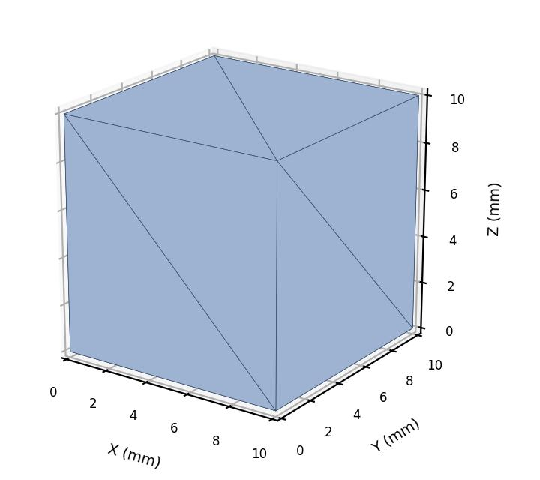
\includegraphics[width=\linewidth]{cube_render.pdf}\\
  {\footnotesize (a) cube\_10}
\end{minipage}\hfill
\begin{minipage}[b]{0.48\columnwidth}
  \centering
  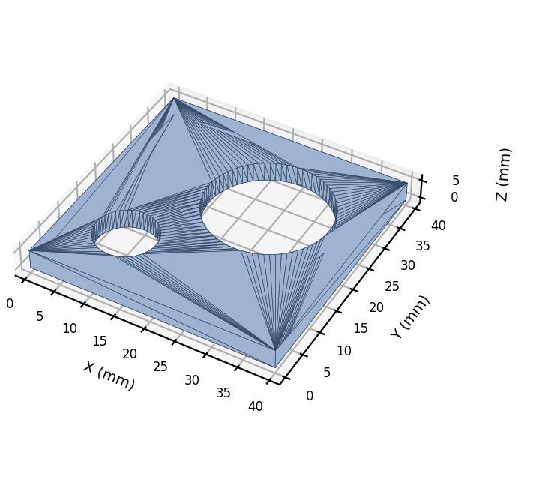
\includegraphics[width=\linewidth]{hole_render.pdf}\\
  {\footnotesize (b) Hole\_Structure}
\end{minipage}
\caption{The two STL test objects. (a) cube\_10, a 10\,mm cube
(12 triangles). (b) Hole\_Structure, a 40$\times$40$\times$5\,mm
plate with 10\,mm and 20\,mm through-holes (532 triangles).
The triangulated top surface of (b) reflects the fan
tessellation present in the source mesh.}
\label{fig:test_objects}
\end{figure}

The two test objects are shown in Figure~\ref{fig:test_objects}.

\begin{figure*}[t]
\centering
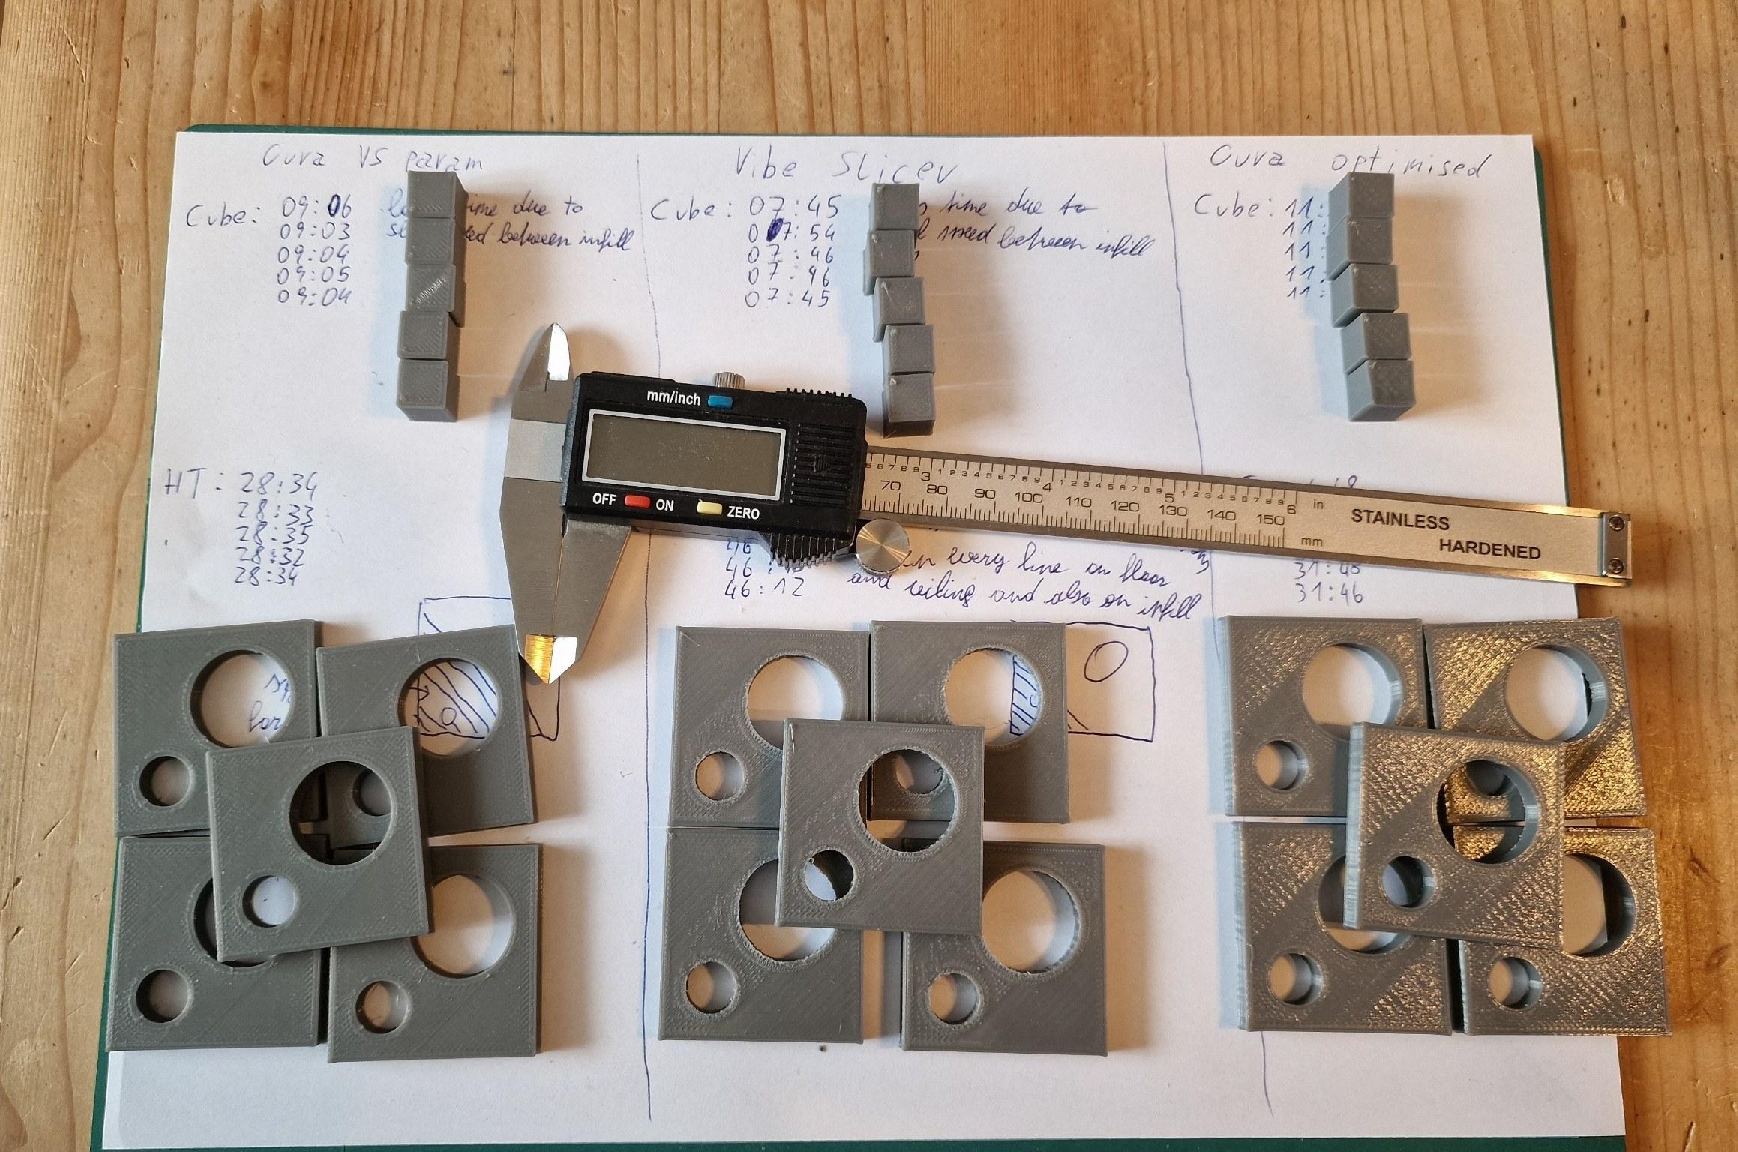
\includegraphics[width=0.82\textwidth]{benchmark_samples.pdf}
\caption{Physical benchmark samples across the three conditions
(left to right: Cura-Matched, Vibe Slicer, Cura-Optimised).
The top row shows the cube\_10 prints (five per condition),
the bottom row the Hole\_Structure plates, and the centre
shows the digital calipers used for measurement.
Handwritten annotations record the per-print times used in
Tables~\ref{tab:cube_cura_vs}--\ref{tab:hole_cura_opt_holes}.}
\label{fig:samples}
\end{figure*}

The printed samples for all three conditions are shown in
Figure~\ref{fig:samples}, alongside the calipers used for
the dimensional measurements.

\subsection{Reference Implementation and Hardware}

For the benchmark tests, Ultimaker Cura (v5.9.0) with two different configurations was used as a reference slicer.
These two Cura configurations  serve the following fundamentally different purposes:

\begin{enumerate}
  \item \textbf{Cura-Matched} (primary comparison): configured
        to match Vibe Slicer's parameters as closely as possible
        (Table~\ref{tab:params}). This is the only \emph{fair}
        head-to-head comparison, since both slicers operate under
        identical process settings and any difference is attributable
        to the slicing and toolpath algorithms themselves.
  \item \textbf{Cura-Optimised} (reference baseline only):
        The authors own parameter preset which is fine tuned on the specific printer for high-quality 1.75mm PLA filaments with a diameter accuracy of $\pm$0.02mm.
        \emph{This parameter set is not a fair comparison against Vibe Slicer}
        because it uses vastly different parameters (lower layer height,
        different speeds and advanced settings) that Vibe Slicer was never
        configured to match. It is reported only to establish what
        best-case Cura output could look like on this printer, and should
        be read as context, not as a competitor to Vibe Slicer.
        Note also that these parameters were not tuned for the generic
        PLA filament used in the tests, which had a diameter accuracy of $\pm$0.05mm, introducing additional hardware-level variability and slight deviations.
\end{enumerate}

Throughout the analysis, all direct claims about how Vibe Slicer
compares to Cura refer to the \textbf{Cura-Matched} condition.
Cura-Optimised results are presented separately
(Section~\ref{sec:opt}) and excluded from the head-to-head
discussion.

Physical prints were produced on a modified Anycubic Chiron
running custom Marlin v1.3.0 firmware, equipped with a 0.4\,mm
68HRC Tool Steel nozzle and generic 1.75\,mm PLA filament ($\pm$0.05\,mm
diameter tolerance). Printed parts were measured with a set of
digital calipers; print time was recorded with a stopwatch.

\begin{table}[H]
\centering
\caption{Benchmark print parameters (identical for both slicers).}
\label{tab:params}
\small
\begin{tabular}{@{}ll@{}}
\toprule
\textbf{Parameter} & \textbf{Value} \\
\midrule
Layer height & 0.2\,mm \\
Offset X & 195\,mm \\
Offset Y & 195\,mm \\
Offset Z & 0\,mm \\
Outer wall lines & 3 \\
Skirtlines & 3 \\
Solid bottom layers & 3 \\
Solid top layers & 3 \\
Infill density & 25\,\% \\
Cooling fan & On after the initial layer at 100 \% \\
Line width & 0.4\,mm \\
Filament diameter & 1.75\,mm \\
Print temperature & 205\,\textdegree{}C \\
Bed temperature & 60\,\textdegree{}C \\
Print speed & 30\,mm/s \\
Z-hop speed & 10\,mm/s \\
Z-hop height & 0.075\,mm \\
Travel speed & 125\,mm/s \\
Print acceleration & 1800\,mm/s$^2$ \\
Retraction distance & 3.0\,mm \\
Retraction speed & 70\,mm/s \\
Retraction min.\ travel & 1.5\,mm \\
\bottomrule
\end{tabular}
\end{table}

\subsection{Metrics}

\textbf{Slicing time} was measured with system-time from
program invocation to output file completion, averaged over five
runs.

\textbf{Print time} is the actual time measured with a stopwatch
from the start of the first layer to the end of the last layer,
averaged over five prints per slicer–object combination.

\textbf{Theoretical dimensional accuracy} was assessed by comparing
nominal object dimensions to the outermost wall centerline coordinates
extracted from the G-code.
Because a line has half its width ($0.2$\,mm) on each side of
the centerline, the expected outer wall centerline for the cube
should lie at $0.2$\,mm and $9.8$\,mm on each axis—not at $0$
and $10$\,mm. Both slicers were verified to comply with this.

\textbf{Practical dimensional accuracy} was assessed by measuring
printed parts with digital calipers at the nominal outer
span of each axis and at the span of each hole, with five prints
per condition.

\subsection{Results}

\subsubsection*{Slicing time}

The slicing time difference between the two tools was too
insignificant to be measured meaningfully on the small test
objects used here. Both the converter and the G-code generator
completed each object in well under a second, and the observed
run-to-run variation was dominated by operating-system latency
(process scheduling, file-system buffering, and start-up overhead)
rather than by any difference in the slicing work itself. Because
this incidental latency was the largest contributor to the measured
duration, no reliable slicing-time comparison could be made at this
scale. A meaningful comparison would require substantially larger
meshes, where the slicing computation dominates the total runtime;
this is discussed further in Section~\ref{sec:discussion}.

\subsubsection*{Theoretical Dimensional Accuracy}

Both Vibe Slicer and Cura (under matched parameters) produce
G-code with wall centerlines offset by exactly $\pm$0.2\,mm
(half the line width) from the nominal face.
No difference was observed in theoretical accuracy for either test
object; the practical difference in printed dimensions therefore
reflects printer hardware-, algorithm- and parameter effects rather than slicer geometry errors.

\subsubsection*{Practical Dimensional Accuracy — cube\_10}

Table~\ref{tab:cube_cura_vs} and Table~\ref{tab:cube_vibe}
report per-print measurements for \textbf{Cura (matched parameters)}
and \textbf{Vibe Slicer}, respectively.

\begin{table}[H]
\centering
\caption{cube\_10 — Cura with matched parameters (mm / mm:ss).}
\label{tab:cube_cura_vs}
\small
\begin{tabular}{@{}ccccc@{}}
\toprule
\textbf{Run} & \textbf{X} & \textbf{Y} & \textbf{Z} & \textbf{Time} \\
\midrule
1 & 10.08 & 10.18 & 10.00 & 09:06 \\
2 & 10.01 & 10.12 & 09.99 & 09:03 \\
3 & 09.98 & 10.09 & 10.02 & 09:04 \\
4 & 10.01 & 10.11 & 10.03 & 09:05 \\
5 & 10.03 & 10.13 & 10.04 & 09:04 \\
\midrule
\textbf{Avg} & \textbf{10.02} & \textbf{10.13} & \textbf{10.02} & \textbf{09:04} \\
\bottomrule
\end{tabular}
\end{table}

\begin{table}[H]
\centering
\caption{cube\_10 — Vibe Slicer (mm / mm:ss).}
\label{tab:cube_vibe}
\small
\begin{tabular}{@{}ccccc@{}}
\toprule
\textbf{Run} & \textbf{X} & \textbf{Y} & \textbf{Z} & \textbf{Time} \\
\midrule
1 & 10.10 & 10.21 & 10.00 & 07:45 \\
2 & 09.92 & 10.04 & 09.99 & 07:54 \\
3 & 10.10 & 10.22 & 10.01 & 07:46 \\
4 & 10.10 & 10.22 & 10.03 & 07:46 \\
5 & 09.94 & 10.06 & 10.00 & 07:45 \\
\midrule
\textbf{Avg} & \textbf{10.03} & \textbf{10.15} & \textbf{10.01} & \textbf{07:47} \\
\bottomrule
\end{tabular}
\end{table}

For the cube, both slicers produce mean outer dimensions within
0.15\,mm of the 10\,mm nominal on all axes, consistent with
typical FDM hardware variability~\cite{gibson2021additive}.
Vibe Slicer shows slightly higher variance on the $X$ axis
(range: 0.18\,mm vs.\ 0.10\,mm for Cura), likely due to the
less optimised seam placement in Vibe Slicer.
Notably, Vibe Slicer's mean print time of 7:47 is 14\,\% faster
than Cura's 9:04, despite identical process parameters—indicating
significant differences in the utilization of travel acceleration and retraction triggering
between the two tools.

\subsubsection*{Practical Dimensional Accuracy — Hole\_Structure (Outer)}

Tables~\ref{tab:hole_cura_out} and \ref{tab:hole_vibe_out}
show outer structure measurements for the 40$\times$40$\times$5\,mm plate.

\begin{table}[H]
\centering
\caption{Hole\_Structure outer — Cura matched (mm / mm:ss).}
\label{tab:hole_cura_out}
\small
\begin{tabular}{@{}ccccc@{}}
\toprule
\textbf{Run} & \textbf{X} & \textbf{Y} & \textbf{Z} & \textbf{Time} \\
\midrule
1 & 39.96 & 40.29 & 04.95 & 28:34 \\
2 & 40.02 & 40.27 & 04.97 & 28:33 \\
3 & 39.98 & 40.26 & 04.95 & 28:34 \\
4 & 40.00 & 40.35 & 04.95 & 28:32 \\
5 & 39.95 & 40.31 & 04.94 & 28:34 \\
\midrule
\textbf{Avg} & \textbf{39.98} & \textbf{40.30} & \textbf{04.95} & \textbf{28:33} \\
\bottomrule
\end{tabular}
\end{table}

\begin{table}[H]
\centering
\caption{Hole\_Structure outer — Vibe Slicer (mm / mm:ss).}
\label{tab:hole_vibe_out}
\small
\begin{tabular}{@{}ccccc@{}}
\toprule
\textbf{Run} & \textbf{X} & \textbf{Y} & \textbf{Z} & \textbf{Time} \\
\midrule
1 & 39.91 & 40.31 & 04.98 & 46:10 \\
2 & 39.95 & 40.39 & 05.00 & 46:14 \\
3 & 39.92 & 40.27 & 04.99 & 46:13 \\
4 & 39.91 & 40.26 & 04.99 & 46:13 \\
5 & 39.91 & 40.28 & 04.97 & 46:12 \\
\midrule
\textbf{Avg} & \textbf{39.92} & \textbf{40.30} & \textbf{04.99} & \textbf{46:12} \\
\bottomrule
\end{tabular}
\end{table}

The most striking result here is print time: Vibe Slicer averages
46:12 versus Cura's 28:33, a 62\,\% increase. The reason for this difference was found to be sub-optimal pathing around the Holes in Vibe Slicer, which lead to a major increase in retractions and empty travel moves. 
Outer $X$ accuracy is marginally worse for Vibe Slicer
($-0.08$\,mm vs.\ $-0.02$\,mm deviation from nominal),
while $Y$ accuracy is comparable for both tools
(both averaging 40.30\,mm, 0.30\,mm above nominal).
The systematic $Y$-axis oversize in both slicers is consistent
with a hardware-level printbed inaccuracy on the test printer.

\subsubsection*{Practical Dimensional Accuracy — Hole\_Structure (Holes)}

Tables~\ref{tab:hole_cura_holes} and \ref{tab:hole_vibe_holes}
report hole diameter measurements.

\begin{table}[H]
\centering
\caption{Hole\_Structure holes — Cura matched (mm).}
\label{tab:hole_cura_holes}
\small
\begin{tabular}{@{}ccccc@{}}
\toprule
\textbf{Run} & \textbf{10mm X} & \textbf{10mm Y} & \textbf{20mm X} & \textbf{20mm Y} \\
\midrule
1 & 09.90 & 10.00 & 19.82 & 20.08 \\
2 & 09.94 & 09.99 & 19.82 & 20.04 \\
3 & 09.93 & 09.97 & 19.86 & 20.00 \\
4 & 09.97 & 09.95 & 19.80 & 20.07 \\
5 & 09.93 & 09.93 & 19.81 & 20.01 \\
\midrule
\textbf{Avg} & \textbf{09.93} & \textbf{09.97} & \textbf{19.82} & \textbf{20.04} \\
\bottomrule
\end{tabular}
\end{table}

\begin{table}[H]
\centering
\caption{Hole\_Structure holes — Vibe Slicer (mm).}
\label{tab:hole_vibe_holes}
\small
\begin{tabular}{@{}ccccc@{}}
\toprule
\textbf{Run} & \textbf{10mm X} & \textbf{10mm Y} & \textbf{20mm X} & \textbf{20mm Y} \\
\midrule
1 & 09.85 & 10.01 & 19.78 & 20.01 \\
2 & 09.84 & 09.95 & 19.79 & 20.00 \\
3 & 09.82 & 10.00 & 19.88 & 20.03 \\
4 & 09.83 & 09.95 & 19.83 & 19.99 \\
5 & 09.80 & 09.97 & 19.90 & 20.04 \\
\midrule
\textbf{Avg} & \textbf{09.83} & \textbf{09.98} & \textbf{19.84} & \textbf{20.01} \\
\bottomrule
\end{tabular}
\end{table}

Hole diameters for both tools are slightly undersized relative
to nominal, which is typical of FDM printing where material
contracts into the hole perimeter~\cite{gibson2021additive}.
Vibe Slicer's 10\,mm hole $X$-axis averages 9.83\,mm
(0.17\,mm undersized) versus Cura's 9.93\,mm (0.07\,mm undersized),
a difference of 0.10\,mm.
For the 20\,mm hole the tools are within 0.02\,mm of each other
on average. The reason for the larger deviations with Vibe Slicer was found to mainly be overall roughness of the Holes, mostly caused by sub-optimal pathing around them. This lead to a major increase in retractions, where small specks of filament were left behind on the inside edges of the Holes. Additionally, Vibe Slicer uses a significantly lower resolution and no path-smoothing compared to Cura for round contours. Overall, all measured dimensions fall within the $\pm$0.3\,mm tolerance typical of consumer FDM hardware.

Table~\ref{tab:summary} provides a consolidated comparison.

\begin{table}[H]
\centering
\caption{Summary: mean deviation from nominal (mm) and mean
print time. Deviation is the mean signed deviation across all
measured axes of each feature (only $X$ and $Y$ diameters for holes).}
\label{tab:summary}
\footnotesize
\begin{tabular}{@{}lcccc@{\hspace{6pt}}|@{\hspace{6pt}}cc@{}}
\toprule
 & \multicolumn{2}{c}{\textbf{Cura matched}} & \multicolumn{2}{c}{\textbf{Vibe Slicer}} & \multicolumn{2}{c}{\textbf{Cura opt.}} \\
\cmidrule(r){2-3}\cmidrule(lr){4-5}\cmidrule(l){6-7}
 & & & & & \multicolumn{2}{c}{\footnotesize\itshape ref.\ only} \\
\textbf{Metric} & Dev. & Time & Dev. & Time & Dev. & Time\\
\midrule
cube outer & $+$0.06 & 09:04 & $+$0.06 & 07:47 & $-$0.01 & 11:32 \\
Hole outer & $+$0.08 & 28:33 & $+$0.07 & 46:12 & $+$0.03 & 31:47 \\
10\,mm hole & $-$0.05 & — & $-$0.10 & — & $-$0.01 & — \\
20\,mm hole & $-$0.07 & — & $-$0.08 & — & $-$0.04 & — \\
\bottomrule
\end{tabular}
\end{table}

Figures~\ref{fig:dev} and~\ref{fig:time} visualise the average
differences across all conditions, with Cura-Optimised hatched.

\begin{figure}[H]
\centering
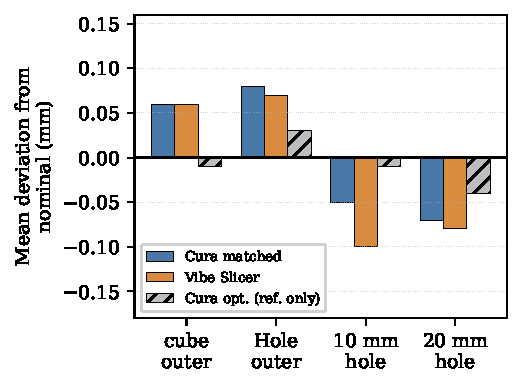
\includegraphics[width=\columnwidth]{bench_deviation.pdf}
\caption{Mean dimensional deviation from nominal (mm) per metric.
Cura-Matched and Vibe Slicer (solid bars) form the head-to-head
comparison; Cura-Optimised (hatched) is the reference baseline.}
\label{fig:dev}
\end{figure}

\begin{figure}[H]
\centering
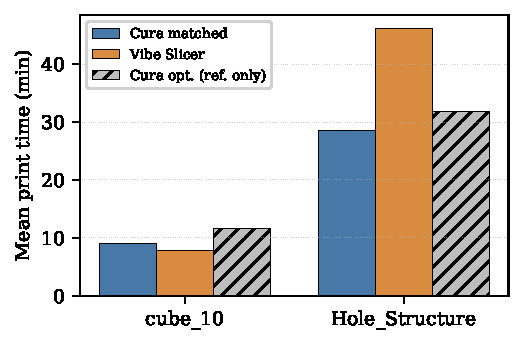
\includegraphics[width=\columnwidth]{bench_time.pdf}
\caption{Mean print time per object. Vibe Slicer matches or
beats Cura-Matched on the simple cube but is substantially slower
on the Hole\_Structure due to missing travel-path optimisation.
Cura-Optimised (hatched) is the reference baseline.}
\label{fig:time}
\end{figure}

\subsection{Cura-Optimised: Reference Baseline}
\label{sec:opt}

The following results report the Cura-Optimised reference baseline,
kept separate from the head-to-head comparison as established in
Section~\ref{sec:eval}.
Tables~\ref{tab:cube_cura_opt} and \ref{tab:hole_cura_opt_out}
report the cube and outer-plate measurements, while Table \ref{tab:hole_cura_opt_holes} reports the hole diameter measurements.

\begin{table}[H]
\centering
\caption{cube\_10 — Cura optimised parameters (mm / mm:ss).}
\label{tab:cube_cura_opt}
\small
\begin{tabular}{@{}ccccc@{}}
\toprule
\textbf{Run} & \textbf{X} & \textbf{Y} & \textbf{Z} & \textbf{Time} \\
\midrule
1 & 09.95 & 10.00 & 10.02 & 11:35 \\
2 & 09.96 & 09.99 & 10.02 & 11:35 \\
3 & 09.96 & 09.98 & 10.00 & 11:27 \\
4 & 09.96 & 09.97 & 10.02 & 11:31 \\
5 & 10.00 & 09.99 & 10.01 & 11:32 \\
\midrule
\textbf{Avg} & \textbf{09.97} & \textbf{09.99} & \textbf{10.01} & \textbf{11:32} \\
\bottomrule
\end{tabular}
\end{table}

\begin{table}[H]
\centering
\caption{Hole\_Structure outer — Cura optimised (mm / mm:ss).}
\label{tab:hole_cura_opt_out}
\small
\begin{tabular}{@{}ccccc@{}}
\toprule
\textbf{Run} & \textbf{X} & \textbf{Y} & \textbf{Z} & \textbf{Time} \\
\midrule
1 & 39.99 & 40.19 & 04.95 & 31:48 \\
2 & 39.98 & 40.16 & 04.96 & 31:45 \\
3 & 39.95 & 40.14 & 04.98 & 31:47 \\
4 & 39.95 & 40.13 & 04.99 & 31:48 \\
5 & 39.99 & 40.17 & 04.96 & 31:46 \\
\midrule
\textbf{Avg} & \textbf{39.97} & \textbf{40.16} & \textbf{04.97} & \textbf{31:47} \\
\bottomrule
\end{tabular}
\end{table}

\begin{table}[H]
\centering
\caption{Hole\_Structure holes — Cura optimised (mm).}
\label{tab:hole_cura_opt_holes}
\small
\begin{tabular}{@{}ccccc@{}}
\toprule
\textbf{Run} & \textbf{10mm X} & \textbf{10mm Y} & \textbf{20mm X} & \textbf{20mm Y} \\
\midrule
1 & 10.00 & 10.01 & 19.92 & 20.00 \\
2 & 09.99 & 10.00 & 19.91 & 20.02 \\
3 & 09.98 & 09.99 & 19.93 & 20.05 \\
4 & 09.99 & 10.00 & 19.88 & 20.00 \\
5 & 10.00 & 10.01 & 19.90 & 20.03 \\
\midrule
\textbf{Avg} & \textbf{09.99} & \textbf{10.00} & \textbf{19.91} & \textbf{20.02} \\
\bottomrule
\end{tabular}
\end{table}

Cura-Optimised achieves near-nominal outer dimensions
($-0.01$\,mm on the cube, $+0.03$\,mm on the plate)
and the closest hole accuracy of all three conditions
($-0.01$ / $-0.04$\,mm). However its print times are significantly longer than that of Cura-Matched: 11:32 on the cube, which is the \emph{longest} time recorded on this object, and 31:47 on the plate. Compared to Cura-Matched this is an increase of 27\,\% on the cube, and 11\,\% on the plate respectively, reflecting the lower layer height and denser
settings in the optimised profile.

% ============================================================
\section{Discussion}
\label{sec:discussion}
% ============================================================

\subsection{Feasibility (RQ1)}

Vibe Slicer successfully produces valid G-code for both test
objects and the printed parts are dimensionally coherent,
demonstrating that AI-assisted development \emph{can} enable an
experienced FDM user with no slicer-development or
geometric-computing background to produce a functionally correct
slicer.
A notable enabling factor was the author's existing FDM domain
knowledge: although unable to implement the geometry algorithms,
the author could reliably recognise incorrect output (malformed
toolpaths, wrong extrusion values, missing layers) and feed
precise corrective feedback to the AI tools. The safety-relevant
G-code ordering and completeness errors discussed in
Section~\ref{sec:prompt_obs} (prompts G8--G11) are a concrete
illustration: recognising that a temperature-reporting command was
absent, the ordering of temperature related control G-code was wrong, that the hotend heating was never deactivated or that layers were started too low required FDM familiarity that the AI did not reliably exhibit. This suggests the
feasibility result may depend partly on the developer's ability
to evaluate output, not solely on the AI's code-generation ability.
The development required 44 recorded prompts (out of well over 150
issued in total) spread over a University semester of part-time
work, with the initial challenge being contour stitching, requiring 4 iterative prompts S1--S4 before correct contour closure on the cube was reached, and later large refactoring prompts for a more robust algorithm enabling hole structures and trying to implement complex shapes S5--S7. The most challenging part however, was the polygon-offset algorithm G23--G31 for small and complex outer wall features and fill boundaries, which was, after creating multiple coordinate blow-ups and other bugs, significantly refactored with S8 and G32--G36, but all prompts ranging from G23--G36 had to ultimately be abandoned due to monthly token budget exhaustion in the final two months of the project while many bugs still remained.

This finding is consistent with survey results~\cite{ziegler2022productivity}
showing AI assistance is effective for boilerplate and moderately
algorithmic tasks, but non-trivial algorithmic knowledge
(here: contour stitching, polygon offsetting, floating-point
tolerance management) still required substantial human-guided iteration.

\subsection{Prompt Engineering Observations}
\label{sec:prompt_obs}

A notable pattern emerged in the development log:
single-line descriptive prompts were sufficient for structural
and I/O tasks (e.g., adding a CLI parameter, splitting files
into packages, adding a G-code command at a specific position)
and produced correct results in one shot in most cases.
In contrast, algorithmic tasks—especially those involving
geometry—required either multi-constraint prompts listing
every edge case explicitly, or iterative diagnosis prompts
describing the observed incorrect behaviour and asking for
the root cause before requesting a fix.
The latter approach (observe wrong output $\to$ ask for cause
$\to$ fix) proved more token-efficient than repeatedly
asking for a complete rewrite, which tended to discard correct
logic along with the bugs.

A further recurring limitation was a lack of context awareness
regarding the conventional ordering and completeness of G-code
command sequences. Several prompts in Table~\ref{tab:prompts_full}
were necessitated solely by such omissions rather than by feature
requests. For instance, prompt G8 was required because the
generated code set the bed temperature (M140) without issuing the
corresponding temperature-reporting command (M105). Prompt G9
addressed a related deficiency in which the relative ordering of
the temperature and reporting commands deviated substantially from
established convention. Prompt G10 was necessary, because at the end of the print sequence, the hotend was never ordered to turn off heating (M104 S0). 
A further example arose at the start of the print sequence: the created G-Code would have started the print at a Z-Axis height of 0.000, which would have in the best case lead to a failed extrusion, but more than likely lead to a crash of the hotend into the Build-plate, requiring the corrective prompt G11.

These shortcomings were predominantly
safety-relevant, and their occurrence during development was
consistent with the author's expectations at the outset of the
project.

The model transition from GPT-5.3 Codex to GPT-5.4-mini
was not a deliberate optimisation: GPT-5.3 Codex was removed
from GitHub Copilot partway through development, forcing all
later work onto GPT-5.4-mini. The two models did, however,
exhibit different characteristics in practice. GPT-5.3 Codex was
faster but more prone to ignoring existing code, while
GPT-5.4-mini was substantially slower but more consistent in respecting the
current project state, requiring less corrective tweaking
afterward. These observed differences are incidental to the
study rather than a controlled comparison.

\subsection{Comparative Performance (RQ2)}
\textbf{Slicing time.}
As reported in Section~\ref{sec:eval}, the slicing-time difference
between the two tools was too small to measure meaningfully on the
bundled test objects: both completed each object in well under a
second, and the run-to-run variation was dominated by
operating-system latency rather than by the slicing work itself.
Slicing time is therefore not a meaningful differentiator at this
scale. A genuine comparison would require production-scale meshes
(millions of triangles), where the slicing computation dominates
total runtime. At that scale, Vibe Slicer's $O(n)$ segment-building
and graph stitching would likely remain competitive with Cura's
compiled C++ at small triangle counts but fall behind at large
counts due to Go's garbage-collection overhead.

\textbf{Dimensional accuracy.}
Theoretical accuracy is identical between all three conditions under
matched parameters.
Practical accuracy reveals a clear hierarchy:
Cura-Optimised $>$ Cura-Matched $\approx$ Vibe Slicer
for outer dimensions, with differences in the 0.05--0.10\,mm
range—all within the hardware noise floor of the test printer without significant parameter tuning.
For hole dimensions, Cura-Optimised achieves near-nominal
accuracy (avg.\ $-0.01$ / $-0.04$\,mm), while Cura-Matched
and Vibe Slicer are both slightly undersized, with Vibe Slicer
approximately 0.05--0.10\,mm more undersized than Cura-Matched.
This is caused by sub-optimal pathing and also likely attributable to Cura's arc-aware hole
approximation producing smoother circular perimeters with more
segments than Vibe Slicer's significantly rougher polygon-offset approach.

\textbf{Print time.}
Vibe Slicer is 14\,\% faster than Cura-Matched on the cube
but 62\,\% slower on the Hole\_Structure.
The cube result is counterintuitive: Vibe Slicer's simpler,
less travel-path-optimised code generates fewer unnecessary
travel moves on a geometry with no internal topology.
For the Hole\_Structure, however, the lack of seam optimisation
and travel-path planning becomes significant across 25 layers
with two internal holes, producing far more unnecessary retraction and
travel moves.
Cura-Optimised is slower than both on the cube (11:32),
reflecting a lower layer height in the optimised profile,
but between the Cura-Matched and Vibe Slicer times
on the plate (31:47), showing that Cura's travel optimisation
partially compensates for its higher feature count.

\subsection{Limitations and Threats to Validity}

The evaluation uses only two axis-aligned test objects on a single
printer. Conclusions about robustness cannot be generalised to
curved surfaces, overhangs, or non-manifold geometry.
The practical accuracy measurements are subject to printer-specific
factors—bed levelling, extruder calibration, ambient temperature—
that are not controlled for here.
None of the three profiles was tuned for the specific PLA
filament batch, introducing additional uncontrolled variability
that may have artificially inflated their outer dimension deviations.
The choice of AI assistant and the prompting strategy adopted may
significantly influence outcome quality; different models or
prompting approaches could yield substantially different results.
The author's prior FDM experience is also a confounding factor:
the ability to recognise incorrect G-code and provide precise
corrective feedback likely accelerated development and improved
outcomes. A developer without this domain knowledge—or one with
geometry expertise but no FDM experience—might encounter very
different difficulties, so the feasibility result should not be
read as applying to an arbitrary inexperienced developer.
Finally, Cura's internal heuristics (seam placement, travel
optimisation, arc detection) cannot be fully disabled,
which likely accounts for the print time and hole accuracy differences.

% ============================================================
\section{Conclusion}
\label{sec:conclusion}
% ============================================================

This paper presented Vibe Slicer, an FDM 3D printer slicer
developed exclusively with AI assistance by an experienced FDM
user who had no prior slicer-development or geometric-computing
experience.
The system implements a complete STL-to-G-code pipeline in Go,
including contour hierarchy extraction with hole support,
configurable wall lines, solid top/bottom layers, zig-zag infill,
skirt, brim, retraction, and cooling fan control,
driven by 44 (30 in live code) conversational prompts across two GPT AI models.

Benchmarking against Ultimaker Cura on two reference objects under
three conditions (Cura-Matched, Vibe Slicer, and Cura-Optimised)
shows that Vibe Slicer achieves theoretical dimensional accuracy
identical to Cura under matched parameters, and practical accuracy
within $\pm$0.3\,mm on outer dimensions and within $\pm$0.2\,mm
on hole diameters.
Print time diverges significantly on the more complex object
($+62$\,\%), highlighting the real cost of missing travel-path
optimisation.

Three conclusions can be drawn from this experiment.
First, AI-assisted development can lower the barrier to entry
for computationally complex software domains, enabling a developer
who understands the problem domain (FDM printing) but not its
implementation (slicing algorithms and geometry) to produce a
working artifact.
Second, the quality of generated code for algorithmic sub-problems
(contour stitching, polygon offsetting) degrades sharply without
carefully crafted multi-constraint prompts and iterative
human-guided diagnosis.
Third, the practical impact of missing higher-level slicer
intelligence (seam placement, travel optimisation) is measurable
in print time but not in dimensional accuracy for simple geometry—
a distinction that may not hold for complex objects.

\textbf{Future work} follows directly from the limitations
identified above and falls into four directions.

First, the largest single cost during development was the
iterative human-guided diagnosis required for the geometry
algorithms—contour stitching and, above all, polygon offsetting.
Retrieval-augmented generation (RAG) over computational-geometry
literature could ground the model in established algorithms
(robust offsetting and contour-orientation methods) rather than
having it re-derive them heuristically across many prompts;
whether this reduces corrective iterations is an open question
the present work is well positioned to motivate.

Second, the polygon-offset routine that ultimately blocked the
hierarchy-aware refactor (prompts G23--G36) should be replaced
with a mature offsetting library such as Clipper2~\cite{clipper2}.
Vibe Slicer's vertex-normal inset degenerates on non-convex and
near-parallel geometry; an integer-arithmetic Minkowski-based
implementation would remove this failure mode and extend
applicability well beyond the simple objects evaluated here.

Third, the most pronounced performance gap—print time on the
Hole\_Structure (Section~\ref{sec:eval})—stems from the absence of
travel-path optimisation and seam placement. Even a greedy
nearest-neighbour ordering of contours with a simple seam
alignment strategy would likely close a substantial fraction of
the 62\,\% print-time gap with Cura-Matched.

Fourth, the evaluation should be extended to a broader benchmark
corpus. The two axis-aligned objects used here deliberately
isolate baseline accuracy and hole handling, but do not exercise
curved surfaces, overhangs, thin walls, or non-manifold input;
a larger and more varied model set would test the contour
pipeline far more thoroughly and allow the findings to be
generalised with greater confidence.

More broadly, the experiment suggests that the boundary of what
AI-assisted development can achieve in a specialist domain is set
less by the model's raw code-generation ability than by the
developer's capacity to specify requirements precisely and
recognise incorrect output—a boundary worth characterising across
domains, developer backgrounds, and prompting strategies.

% ---- Acknowledgements ----
\subsection*{Acknowledgements}

The author thanks Univ.-Prof. Dipl.-Inform. Dr.-Ing. Christoph Kirsch, who was the lecturer in the Advanced Systems Engineering class at the University of Salzburg for their feedback
and guidance. GPT-5.3 Codex and GPT-5.4-mini were
used as primary AI development assistants throughout this project.
Claude Sonnet and Opus were used for paper writing assistance.

\onecolumn
\appendix
\section{Prompt Development Log}
\label{app:prompts}

This appendix documents the prompts that contributed directly to
the final result. Table~\ref{tab:prompts_full} reproduces these
44 prompts \emph{verbatim} as they were written, together with
the model used and the outcome of each. They are a curated subset:
well over 150 prompts were issued in total, but the majority led
to unproductive cycles (a fix for one problem causing a regression
elsewhere) after which the working tree was reset, and only the
prompts on the path to the working code are retained here (exceptions being G23-G36). 
Prompts are numbered sequentially within each component
(S = stl\_to\_json\_converter [STL-to-JSON converter], G = create\_g\_code [G-code generator]).

\vspace{6pt}
\footnotesize
\setlength{\LTleft}{0pt}
\setlength{\LTright}{0pt}

\begin{longtable}{@{}p{0.6cm}p{1.5cm}p{11.0cm}p{2.7cm}@{}}
\caption{Recorded prompt log: the 44 prompts on the path to the
final result, reproduced verbatim as issued, with model and
outcome. A larger pool of exploratory prompts that led to
reset cycles is not shown.}
\label{tab:prompts_full}\\
\toprule
\textbf{ID} & \textbf{Model} & \textbf{Prompt (verbatim)} & \textbf{Outcome} \\
\midrule
\endfirsthead
\multicolumn{4}{@{}l}{\footnotesize\itshape Table~\ref{tab:prompts_full} continued from previous page}\\
\toprule
\textbf{ID} & \textbf{Model} & \textbf{Prompt (verbatim)} & \textbf{Outcome} \\
\midrule
\endhead
\midrule
\multicolumn{4}{r@{}}{\footnotesize\itshape continued on next page}\\
\endfoot
\bottomrule
\endlastfoot

\multicolumn{4}{@{}l}{\textbf{STL-to-JSON converter}}\\
\midrule
S1 & GPT-5.3 Codex & Create a go file that takes a file in STL format as input, slices the object in the STL file every 0.2mm, starting from the bottom and converts the resulting 2D coordinates into an array of x and y coordinates. & Working; Bug present: 8 points per layer instead of 4 \\
\addlinespace
S2 & GPT-5.3 Codex & Why does go run . -in .\textbackslash cube\_10.stl produce 8 points after layer height 0.2, when the object is a cube that should only have 4 points? & Cause identified: missing post-steps \\
\addlinespace
S3 & GPT-5.3 Codex & Perform the following suggested post-steps after sliceTriangles and update readme.md with the new logic:\newline
[1]~build contour segments from triangle intersections \newline
[2]~stitch ordered loops \newline
[3]~remove collinear intermediate points (polygon simplification) & Implemented; Bug present: wrong ordering of coordinates
\\
\addlinespace
S4 & GPT-5.3 Codex & Order the output coordinates of stl\_to\_json\_converter in the form of a clockwise toolpath, so x = 0, y = 0, then x = 0, y = 10, then x = 10, y = 10 and so on. & Implemented; working as intended \\
\addlinespace
S5 & GPT-5.4-mini & Fix the weaknesses in stl\_to\_json\_converter found in the README. In particular, fix the: loss of contour hierarchy, weak handling of non-manifold geometry, sensitivity to floating-point precision and add support for more complex shapes. Do this while still retaining the tool-path like ordering that is currently implemented. & Partial implementation; coordinate blow-ups on complex shapes; Cause identified \\
\addlinespace
S6 & GPT-5.4-mini & Perform the following changes:
\begin{enumerate}
	\item{Refactor stl\_to\_json\_converter so the STL-to-2D-layer pipeline is topology-aware instead of relying mainly on flattened points}
	\item{Compute triangle-plane intersections with scale-aware tolerances derived from model bounds and layer height}
	\item{Deduplicate nearly coincident intersection vertices using snapping or tolerance-based merging}
	\item{Build an explicit segment graph from intersection segments before contour reconstruction}
	\item{Replace heuristic path walking with deterministic contour-cycle extraction}
	\item{Preserve multiple disjoint loops, nested holes, and open chains as first-class structures in the JSON output}
	\item{Normalize and simplify closed contours by removing duplicate points and collinear runs} 

	\item{Validate closed contours before export: 
		\begin{enumerate}
			\item{reject zero-length edges}
			\item{reject self-intersections}
			\item{reject invalid or ambiguous cycles} 
			\item{ensure consistent winding and nesting} 
		\end{enumerate}}
	\item{Handle co-planar triangles, duplicate triangle contributions, and non-manifold edge cases defensively}
	\item{Use adaptive tolerances instead of a single fixed epsilon wherever possible}
	\item{On unstable or ambiguous geometry, fail safely by dropping only the invalid local structure rather than emitting runaway coordinates or invalid polygons}
	\item{Keep the structured contours tree as the authoritative representation and treat flattened points as a compatibility view}
	\item{Add regression tests for: 
		\begin{enumerate}
			\item{nearly coincident vertices}
			\item{shallow-angle edges}
			\item{co-planar triangles}
			\item{holes}
			\item{open chains}
			\item{non-manifold or thin-feature input}
		\end{enumerate}} 
\end{enumerate} & Mostly implemented; Re-run prompt \\
\addlinespace
S7 & GPT-5.4-mini & [Re-run of prompt S6, additionally refactoring create\_g\_code to consume the new structured input.] & Near-correct; minor edge/top-layer bugs \\
\addlinespace
S8 & GPT-5.4-mini & Fully coplanar triangles are being converted into only two of their three edges, which turns a cap triangulation into incomplete fragments. Replace that heuristic with a ``emit all three edges and let shared edges cancel'' behavior. & Top-layer bug resolved; Edge bug still present \\
\midrule
\multicolumn{4}{@{}l}{\textbf{G-code generator}}\\
\midrule
G1 & GPT-5.3 Codex & Create a new go file called ``create\_g\_code'' that takes the json coordinate input from stl\_to\_json\_converter and creates GCODE for an FDM Type 3D Printer in a .gcode file. The new go file should include offset parameters for:
\begin{enumerate}
	\item{Start GCODE = that gets added to the beginning of the resulting .gcode file}
	\item{End GCODE = that gets appended to the end of the resulting .gcode file}
	\item{Line width = that represents the width of the printers nozzle line in mm}
	\item{print temperature = that represents the printhead temperature in Celsius}
	\item{build plate temperature = that represents the temperature of the build plate in Celsius}
	\item{print speed = that represents the speed for printing on the x and y axis in mm/s}
	\item{z hop speed = that represents the speed for the z axis in mm/s}
	\item{travel speed = that represents the speed for travel moves in mm/s}
	\item{print acceleration = that represents the acceleration for printer moves in mm/s\^{}2} \item{retraction distance = that represents the distance to retract the filament from the printhead during travel moves in mm}
	\item{retraction speed = that represents how fast the filament is retracted in mm/s}
	\item{retraction minimum travel = that represents how far a travel move has to be in order to trigger the retraction process in mm} 
\end{enumerate} & Implemented \\
\addlinespace
G2 & GPT-5.3 Codex & Remove the new offset values from the stl\_to\_json\_converter class main method and instead add them to the create\_g\_code main function. The stl\_to\_json\_converter should only produce a json file that can then be read by the create\_g\_code class. They should be two separate classes. Additionally, add z-hop-height and filament-diameter parameters. & Implemented \\
\addlinespace
G3 & GPT-5.3 Codex & Add a short section in README.md called ``Two-step workflow'' with copy/paste commands for both tools end-to-end. & Implemented \\
\addlinespace
G4 & GPT-5.3 Codex & Move stl\_to\_json\_converter and stl\_to\_json\_converter\_test to a separate folder called ``stl\_to\_json\_converter''. & Implemented \\
\addlinespace
G5 & GPT-5.3 Codex & Remove the old create\_g\_code and create\_g\_code\_test files in the root, since they are now located in their own folder. & Implemented \\
\addlinespace
G6 & GPT-5.3 Codex & Add x, y, and z axis offset parameters to the pre-existing parameters in create\_g\_code to enable an offset of the print on the build-plate. & Implemented \\
\addlinespace
G7 & GPT-5.3 Codex & Change the startGCode insertion position in create\_g\_code to be inserted after M109. & Implemented \\
\addlinespace
G8 & GPT-5.3 Codex & Insert M105 after M140 in create\_g\_code. & Implemented \\
\addlinespace
G9 & GPT-5.3 Codex & Order the commands M140, M190, M105, M104 and M109 in create\_g\_code in the following way. M140 $\rightarrow$ M105 $\rightarrow$ M190 $\rightarrow$ M104 $\rightarrow$ M105 $\rightarrow$ M109. & Implemented \\
\addlinespace
G10 & GPT-5.3 Codex & In create\_g\_code before the insertion of endGCode, add M140 S0. After the endGCode insertion, add another M104 S0. & Implemented \\
\addlinespace
G11 & GPT-5.4-mini & In create\_g\_code the initial layer height right now is Z0.000. This results in a crash of the toolhead. Set the initial layer height to the layer\_height\_mm specified in the converted JSON input file. & Implemented; Bug present: Printed object end-height now too high \\
\addlinespace
G12 & GPT-5.4-mini & In create\_g\_code, the initial layer height offset now causes the resulting gcode layers to be too high by the amount of layer height. & Implemented; working as intended \\
\addlinespace
G13 & GPT-5.4-mini & In create\_g\_code add the possibility to have a closed bottom and top layer that is printed in a right-hand 45 degree angle in relation to the x-axis/front of the print. There should also be the possibility to adjust the number of these fully printed layers with 2 separate parameters for bottom and top. If at any location (bottom or top) there is more than 1 layer set, the 45 degree angle should alternate for this location between left-hand and right-hand, starting from right hand at the first printed layer. & Implemented \\
\addlinespace
G14 & GPT-5.4-mini & In create\_g\_code, add the possibility to choose the number of solid outer wall lines. For this, add a parameter with a minimum value of 1 (just the outer wall). The additional solid outer walls should be printed inwards, in order to retain dimensional accuracy. & Implemented; Bug present: Line width not considered - printed object outside dimensions too large \\
\addlinespace
G15 & GPT-5.4-mini & In create\_g\_code, the currently generated outer dimensions in the gcode are inaccurate, since the parameter lineWidth is not considered for the out most dimension. Change the code in such a way, that the lineWidth parameter is considered by half of its given value. For example in the case of cube\_10 which is 10x10x10mm and a lineWidth of 0.4, the left outer wall for a dimensionally accurate print is not at 180 (which is currently the case), but at 180.2. & Implemented; working as intended \\
\addlinespace
G16 & GPT-5.4-mini & In create\_g\_code, the toolpath for the floor and ceiling lines are currently intersecting the toolpath of the inner most wall line. This should however not be the case. The calculation should consider the lineWidth parameter divided by 2 in order to stop this intersection. Do not make any changes to the wall lines, make the changes in the floor and ceiling calculations. & Implemented; Bug present: Small gap present on edges \\
\addlinespace
G17 & GPT-5.4-mini & In create\_g\_code on both floor and ceiling prints, at the end of each layer, there now exists a small gap. Find out why that is and make the necessary changes to fill this gap as well. & Implemented; working as intended \\
\addlinespace
G18 & GPT-5.4-mini & In create\_g\_code, add the possibility to print infill in a Zig-Zag pattern. The infill print should start after the last floor layer was printed and end at the last layer before the ceiling is printed. For this, add to the existing parameters the boolean parameter infill, which controls if an infill should be printed (true if yes) and the parameter infill density, which represents the density of the infill to be generated in \% (100\% would be solid, 0\% would be no infill at all). & Implemented; Bug present: No Zig-Zag - only prints in one direction \\
\addlinespace
G19 & GPT-5.4-mini & In create\_g\_code, alternate the infill the same way as the floor and ceiling print directions, i.e. 45deg lefthand, then 45deg righthand at the next layer. & Implemented; working as intended \\
\addlinespace
G20 & GPT-5.4-mini & In create\_g\_code, add support for an extruder cooling fan (M106). For this, add to the existing parameters the boolean parameter cooling fan, which controls if the cooling fan should be used, the integer parameter cooling fan layer, which sets the layer at which the cooling fan should be turned on and the parameter cooling fan speed, which represents the speed to set the cooling fan to in \% (100\% would be 255, 0\% would be 0). At the end of the print after the M140 S0 command, add M107 if the parameter cooling fan was set to true. & Implemented \\
\addlinespace
G21 & GPT-5.4-mini & In create\_g\_code, add support for a brim, which is an extension of the printed surface area of the initial layer to improve bed adhesion. For this, add a boolean named brim, which if set to true, enables the brim print. Additionally, add the parameter brimLines which represents the amount of additional lines to print for the brim. For the brim lines, consider all the parameters like line width etc. that would be considered on the regular initial layers wall print. & Implemented \\
\addlinespace
G22 & GPT-5.4-mini & In create\_g\_code, add support for a skirt, which is one-, or multiple lines printed around the outmost line of the printed object on the initial layer. The purpose of this is to prime the hotend nozzle, so this should always be printed first before printing anything else. For this, add the boolean parameter skirt, which if set to true, enables the skirt print. Additionally, add the parameter skirtLines, which defines the amount of skirt lines to print. For the skirt lines, consider all the parameters like line width etc. that would be considered on the regular initial layers wall print. The innermost skirt line should also have at least a 5mm gap to the outermost printed wall line, or if a brim is enabled, the outermost brim line. & Implemented \\
\midrule
\multicolumn{4}{@{}p{15.8cm}@{}}{\itshape Prompts G23--G36 correspond to the hierarchy-aware offset refactor prompted by the failed attempt at converter prompt S5. They were re-approached several times but are not included in the final code, since the author ran out of AI tokens with unresolved bugs (coordinate blow-ups and spurious print moves on more complex objects) that rendered the resulting G-code unusable or dangerous in some cases.}\\
\midrule
G23 & GPT-5.4-mini & Update create\_g\_code with the added contours hierarchy. & Abandoned; Multiple bugs present \\
\addlinespace
G24 & GPT-5.4-mini & Make create\_g\_code fully hierarchy-aware for walls/fills, so that holes are handled explicitly. & Abandoned; Multiple bugs present \\
\addlinespace
G25 & GPT-5.4-mini & In create\_g\_code, the floor and infill now uses the outer most wall as a start and end point. This is not correct. Use the inner most wall as reference for this. Extruding lines should not overlap. Also take line width into account for this. & Abandoned; Multiple bugs present \\
\addlinespace
G26 & GPT-5.4-mini & In create\_g\_code, the floor/ceiling and infill are now not touching the outer walls. This should however be the case. Consider using linewidth/2 to prevent this. & Abandoned; Multiple bugs present \\
\addlinespace
G27 & GPT-5.4-mini & In create\_g\_code, the the floor/ceiling and infill are now overlapping the inner most wall line. They should however just touch the outer most part of said line. A line is linewidth thick, meaning linewidth/2 on each side. & Abandoned; Multiple bugs present \\
\addlinespace
G28 & GPT-5.4-mini & In xyzcube.gcode, there are erroneous print moves from layer 20 onward that far exceed the coordinates in xyzcube.json. Find the root cause of this. & Supposedly diagnosed by AI \\
\addlinespace
G29 & GPT-5.4-mini & Pinpoint the exact wall layer/offset depth where the first bad vertex is created. & Supposedly diagnosed by AI \\
\addlinespace
G30 & GPT-5.4-mini & Pinpoint which two adjacent edges around point 12 make the line intersection blow up. & Supposedly diagnosed by AI\\
\addlinespace
G31 & GPT-5.4-mini & Find a geometric safeguard to prevent the two adjacent almost parallel offset edges to blow up the line intersection and fix it in code. & Abandoned; Multiple bugs present; No progress - initiated refactor of stl\_to\_json\_converter with AI suggestions (S6--S8) after token budget reset \\
\addlinespace
G32 & GPT-5.4-mini & Refactor create\_g\_code to take the new more robust input from stl\_to\_json\_converter. Keep all of the parameters (flag) logic. & Abandoned; Top-layer bug gone; letter-edge and infill bugs remain \\
\addlinespace
G33 & GPT-5.4-mini & [Long multi-section spec.]
\begin{enumerate}
	\item {Inspect the current fill pipeline in create\_g\_code:} 
	\begin{enumerate}
		\item{Trace how emitInfill(...) and emitSolidFill(...) build fill segments}
		\item{Identify where contour offsets, scanline intersections, and segment pairing happen}
	\end{enumerate}
	\item{Switch fill generation to use structured contours:}
	\begin{enumerate}
		\item{Treat contours as the authoritative layer geometry}
		\item{Avoid using flattened points for fill construction except as a fallback}
	\end{enumerate}
	\item{Preserve the fill control parameter:}
	\begin{enumerate}
		\item{Keep -infill-density as the user-facing control for infill spacing}
		\item{Continue deriving spacing from density and line width, but through safer geometry handling}
	\end{enumerate}
	\item{Build conservative fill boundaries:}
	\begin{enumerate}
		\item{Generate fill regions from validated closed contours}
		\item{Use adaptive tolerances when offsetting boundaries}
		\item{Reject unstable or degenerate offsets instead of forcing them through}
	\end{enumerate}
	\item{Replace simple intersection pairing:}
	\begin{enumerate}
		\item{Stop pairing scanline intersections only by sorted order}
		\item{Use a topology-aware method that respects polygon nesting and parity}
		\item{Ensure fill segments stay inside valid printable regions}
	\end{enumerate}
	\item{Clip fill against nested contours:}
	\begin{enumerate}
		\item{Keep holes empty}
		\item{Make sure infill does not cross outer walls or bridge through concavities incorrectly}
	\end{enumerate}
	\item{Handle ambiguous geometry safely:}
	\begin{enumerate}
		\item{If a local region becomes invalid, drop only that region}
		\item{Do not generate runaway fill segments or invalid extrusion paths}
	\end{enumerate}
	\item{Keep wall and fill coordination consistent:}
	\begin{enumerate}
		\item{Ensure outer-wall offsets and fill boundaries agree}
		\item{Prevent fill from invading the wall-perimeter area}
	\end{enumerate}
	\item{Add regression tests:}
	\begin{enumerate}
		\item{Concave middle-layer contours}
		\item{Narrow channels near walls}
		\item{Nested holes}
		\item{Near-degenerate offsets}
		\item{High-density infill cases}
		\item{Transition layers where fill meets walls}
	\end{enumerate}
	\item{Verify against the existing G-code output:}
	\begin{enumerate}
		\item{Compare generated paths on the problematic calibration model}
		\item{Confirm infill stays inside the intended shape at middle layers}
	\end{enumerate}
\end{enumerate} & Abandoned; Infill no longer pokes through - bug resolved; Top layer now overlaps ceiling features; Letter-edge bug remains \\
\addlinespace
G34 & GPT-5.4-mini & [Long multi-section spec.] \newline
Refactor the wall-offset geometry in create\_g\_code.go to prevent runaway corner intersections on sharp or nearly parallel vertices while preserving existing slicer behavior and CLI parameters. \newline
Scope:
\begin{enumerate}
	\item{Focus on the wall generation path used by:}
	\begin{enumerate}
		\item{emitOuterWalls(...)}
		\item{offsetPolygon(...)}
		\item{intersectLines(...)}
		\item{isReasonableOffsetVertex(...)}
	\end{enumerate}
	\item{Do not change brim/skirt behavior unless needed as a shared helper, and do not alter public flag names or meanings} 
\end{enumerate}
[\textbf{Prompt continues on next page}] & Abandoned; Bugs still present - Top layer overlapping ceiling features, still produced extended edges on letters \\
\addlinespace
G34 & GPT-5.4-mini & [\textbf{Continued prompt from previous page}] \newline
Required changes:		
\begin{enumerate}
	\item{Replace pure miter-only corner construction with a bounded offset-join strategy:}
	\begin{enumerate}
		\item{Keep the current line-offset approach for ordinary corners}
		\item{Introduce a miter limit check for each corner intersection}
		\item{Measure miter length relative to the local edge length / offset distance}
		\item{If the miter exceeds the configured threshold or the lines are near-parallel, fall back to a safer join}
	\end{enumerate}
	\item{Add a safe fallback join:}
	\begin{enumerate}
		\item{Preferred fallback: bevel join between the two offset edges}
		\item{Alternative acceptable fallback: reject the local corner and return a non-extended offset loop failure for that layer/loop}
		\item{The fallback must avoid generating spikes or points far outside the local polygon neighborhood}
	\end{enumerate}
	\item{Strengthen intersection robustness:}
	\begin{enumerate}
		\item{In intersectLines(...), treat near-parallel offset edges as unstable earlier}
		\item{Add a tolerance-aware parallelism check based on local scale, not only a fixed epsilon}
		\item{Prevent producing extremely large coordinates when the denominator is small but nonzero}
	\end{enumerate}
	\item{Tighten offset vertex validation:}
	\begin{enumerate}
		\item{Update isReasonableOffsetVertex(...) to reject corners with excessive miter extension}
		\item{Compare the intersection point against the original vertex and local edge lengths}
		\item{Make the acceptance threshold scale-aware instead of using only a very broad bounding box}
	\end{enumerate}
	\item{Keep the offset loop valid or fail safely:}
	\begin{enumerate}
		\item{If one corner in an offset loop is unstable, do not emit a runaway polygon}
		\item{Either:}
		\begin{enumerate}
			\item{degrade the local corner with a bevel join, or}
			\item{discard that offset loop and fall back to the source contour where appropriate} 
		\end{enumerate}
		\item{Never emit a perimeter that extends beyond the object footprint due to a bad miter}
	\end{enumerate}
	\item{Preserve compatibility:}
	\begin{enumerate}
		\item{Keep the current CLI flags unchanged}
		\item{Keep the existing insetPolygon(...) / outsetPolygon(...) entry points}
		\item{Maintain current behavior for normal convex polygons and non-problematic corners}
	\end{enumerate}
\end{enumerate}
Implementation details:	
\begin{enumerate}
	\item{Add a helper such as:}
	\begin{enumerate}
		\item{cornerMiterLength(...)}
		\item{shouldBevelJoin(...)}
		\item{buildBevelJoin(...)}
	\end{enumerate}
	\item{Use local geometry:}
	\begin{enumerate}
		\item{previous edge length}
		\item{next edge length}
		\item{offset distance}
		\item{turn angle}
	\end{enumerate}
	\item{Use a clear threshold such as:}
	\begin{enumerate}
		\item{miter limit in multiples of the offset distance}
		\item{or a ratio against the shorter adjacent edge}
	\end{enumerate}
	\item{Prefer deterministic handling, not heuristic retries}
\end{enumerate}
Validation requirements:
\begin{enumerate}
	\item{Add or update tests to cover:}
	\begin{enumerate}
		\item{sharp convex corners that previously produced spikes}
		\item{nearly parallel adjacent edges}
		\item{very small local angles}
		\item{ordinary square/cube outlines to ensure no regression} 
		\item{loops that should be rejected safely instead of overextended}
	\end{enumerate}
\end{enumerate} 
Acceptance criteria:
\begin{enumerate}
	\item{No wall offset should extend beyond the intended object bounds because of a corner spike}
	\item{Normal perimeters still print correctly}
	\item{The fix must be deterministic and not depend on manual tuning per model}
	\item{Existing slicer parameters and G-code generation flow remain intact}
\end{enumerate} & Abandoned; Bugs still present - Top layer overlapping ceiling features, still produced extended edges on letters \\
\addlinespace
G35 & GPT-5.4-mini & Add a miter limit at the corner join in offsetPolygon(...). If the miter is too long or the edges are nearly parallel, fall back to a bevel join, or reject that offset loop safely. Keep outerWallLines unchanged. & Abandoned; Bugs still present - Top layer overlapping ceiling features, still produced extended edges on letters \\
\addlinespace
G36 & GPT-5.4-mini & [Long multi-section spec.] \newline
Refactor the wall-offset geometry in create\_g\_code.go to prevent runaway corner intersections on sharp or nearly parallel vertices. The current miter-based corner construction is still producing outward spikes on some contours, so the offset logic must be made more robust. \newline
Goals:
\begin{enumerate}
	\item{Prevent long miter spikes on sharp corners}
	\item{Replace the current “accept the line intersection if it looks reasonable” behavior with a much stricter miter limit}
	\item{Use a true bevel / clip fallback when the miter limit is exceeded}
	\item{If the local geometry is unstable, reject only that loop locally and fail safely}
	\item{Preserve outerWallLines, all CLI flags, and the current overall slicer flow}
\end{enumerate}
Required changes:
\begin{enumerate}
	\item{Use a stricter miter limit:}
	\begin{enumerate}
		\item{In offsetPolygon(...), keep the current offset-line construction for normal corners}
		\item{Add a much stricter miter limit at each corner}
		\item{Measure the corner miter against:}
		\begin{enumerate}
			\item{the offset distance}
			\item{the shorter adjacent edge}
			\item{and local contour scale} 
		\end{enumerate}
		\item{If the miter exceeds the allowed threshold, do not accept it} 
	\end{enumerate} 
	\item{Replace the current fallback with a true bevel / clip fallback:}
	\begin{enumerate}
		\item{Do not just return the raw offset endpoints unless they are actually clipped and safe}
		\item{Implement a proper bevel-style join or clipped corner fallback that:}
		\begin{enumerate}
			\item{follows the offset edges}
			\item{does not extend beyond the local contour neighborhood}
			\item{and keeps the polygon valid} 
		\end{enumerate}
		\item{If even the bevel fallback cannot be made safe, reject that offset loop locally} 
	\end{enumerate}
	\item{Strengthen near-parallel detection:}
	\begin{enumerate}
		\item{In intersectLines(...), treat nearly parallel offset directions as unstable earlier}
		\item{Use a tolerance-aware parallelism test based on local scale, not only a fixed epsilon}
		\item{Prevent large coordinate blowups when the line intersection denominator is small but nonzero} 
	\end{enumerate}
	\item{Use a robust polygon offset approach:}
	\begin{enumerate}
		\item{Prefer a robust polygon offset algorithm/library over hand-rolled miter intersection if possible}
		\item{If an external library is introduced, use it for:}
		\begin{enumerate}
			\item{inset / outset generation}
			\item{safe bevel / join handling}
			\item{and cleanup of invalid offset geometry} 
		\end{enumerate}
		\item{If no library is added, implement the offset using a more robust polygon-clipping/offsetting approach instead of relying solely on line-line intersections} 
	\end{enumerate}
	\item{Harden vertex validation:}
	\begin{enumerate}
		\item{Update isReasonableOffsetVertex(...) so it:}
		\begin{enumerate}
			\item{rejects excessive miter extension}
			\item{compares the candidate point against the original corner and adjacent edge lengths}
			\item{and uses scale-aware thresholds} 
		\end{enumerate}
		\item{Avoid broad bounding-box-only acceptance rules}
	\end{enumerate}
	\item{Fail safely and locally:}
	\begin{enumerate}
		\item{If one corner in an offset loop is unstable, do not emit a runaway polygon}
		\item{Reject only that local offset loop when necessary}
		\item{Never emit wall geometry that extends beyond the intended object footprint due to a bad corner join} 
	\end{enumerate}
	\item{Preserve compatibility}
	\begin{enumerate}
		\item{Keep insetPolygon(...) and outsetPolygon(...) as the entry points}
		\item{Keep outerWallLines unchanged}
		\item{Keep all CLI flag names and meanings unchanged}
		\item{Preserve the current wall-generation flow for normal convex polygons} 
	\end{enumerate}
\end{enumerate}
[\textbf{Prompt continues on next page}] & Abandoned; Incomplete - AI token budget exhausted \\
\addlinespace
G36 & GPT-5.4-mini & [\textbf{Continued prompt from previous page}] \newline
Suggested implementation direction:
\begin{enumerate}
	\item{Use one of these approaches:}
	\begin{enumerate}
		\item{Preferred: switch to a robust polygon offset library / algorithm with join styles and miter limits} 
		\item{Alternative: implement a stricter custom offset pipeline with:}
		\begin{enumerate}
			\item{bounded miters}
			\item{proper bevel clipping}
			\item{scale-aware near-parallel rejection}
			\item{and safe fallback to loop rejection} 
		\end{enumerate}
	\end{enumerate}
\end{enumerate}
Validation requirements:
\begin{enumerate}
	\item{Add or update tests for:}
	\begin{enumerate}
		\item{sharp convex corners that previously produced spikes}
		\item{nearly parallel adjacent edges}
		\item{very small local angles}
		\item{ordinary square/cube outlines to ensure no regression}
		\item{loops that should be rejected safely instead of overextended} 
	\end{enumerate}
\end{enumerate}
Acceptance criteria:
\begin{enumerate}
	\item{No wall offset should extend beyond the intended object bounds because of a corner spike}
	\item{Normal perimeters still print correctly}
	\item{The fix is deterministic}
	\item{Repeated wall offsets remain safe}
	\item{Existing slicer parameters and G-code generation flow remain intact}
\end{enumerate} & Abandoned; Incomplete - AI token budget exhausted\\
\end{longtable}
\twocolumn

% ---- References ----
\begin{thebibliography}{99}

\bibitem{guo2013additive}
N.~Guo and M.~C.~Leu,
``Additive manufacturing: Technology, applications and research needs,''
\textit{Frontiers of Mechanical Engineering},
vol.~8, no.~3, pp.~215--243, 2013.

\bibitem{cura}
Ultimaker BV,
``Ultimaker Cura,''
[Online]. Available: \url{https://ultimaker.com/software/ultimaker-cura}.
[Accessed: June 2026].

\bibitem{prusaslicer}
Prusa Research,
``PrusaSlicer,''
[Online]. Available: \url{https://github.com/prusa3d/PrusaSlicer}.
[Accessed: June 2026].

\bibitem{chen2021codex}
M.~Chen \textit{et al.},
``Evaluating large language models trained on code,''
\textit{arXiv preprint arXiv:2107.03374}, 2021.

\bibitem{jiang2023survey}
J.~Jiang, F.~Wang, J.~Shen, S.~Kim, and S.~Kim,
``A survey on large language models for code generation,''
\textit{arXiv preprint arXiv:2406.00515}, 2024.

\bibitem{jimenez2023swebench}
C.~E.~Jimenez \textit{et al.},
``SWE-bench: Can language models resolve real-world GitHub issues?,''
\textit{arXiv preprint arXiv:2310.06770}, 2023.

\bibitem{gibson2021additive}
I.~Gibson, D.~Rosen, B.~Stucker, and M.~Khorasani,
\textit{Additive Manufacturing Technologies}, 3rd~ed.
Springer, 2021.

\bibitem{jin2020connections}
Z.~Jin, Z.~Zhang, and G.~X.~Gu,
``Achieving better connections between deposited lines in
additive manufacturing via machine learning,''
\textit{Mathematical Biosciences and Engineering},
vol.~17, no.~4, pp.~3382--3394, 2020.
DOI: 10.3934/mbe.2020191.

\bibitem{clipper2}
A.~Johnson,
``Clipper2: Polygon clipping and offsetting library,''
[Online]. Available: \url{https://github.com/AngusJohnson/Clipper2}.
[Accessed: June 2026].

\bibitem{radford2019gpt2}
A.~Radford \textit{et al.},
``Language models are unsupervised multitask learners,''
\textit{OpenAI Blog}, 2019.

\bibitem{copilot}
GitHub Inc.,
``GitHub Copilot,''
[Online]. Available: \url{https://github.com/features/copilot}.
[Accessed: June 2026].

\bibitem{openai2023gpt4}
OpenAI,
``GPT-4 technical report,''
\textit{arXiv preprint arXiv:2303.08774}, 2023.

\bibitem{ziegler2022productivity}
A.~Ziegler \textit{et al.},
``Productivity assessment of neural code completion,''
in \textit{Proc.\ DL4C Workshop at ICLR}, 2022.

\end{thebibliography}

\end{document}
